\chapter{Diagnóstico situacional}

\section{Análisis externo}

\subsection{Análisis del entorno}
\subsubsection{Análisis Político}
Actualmente en el Perú se tiene una legislación de libre mercado. A pesar de que nos encontramos en pleno proceso electoral, las propuestas de los dos candidatos restantes no alteraran este hecho. Debido a que nuestro emprendimiento es digital, no hay una entidad reguladora, más allá de los impuestos que hay que tributar. Actualmente se está poniendo énfasis en el financiamiento de proyectos tecnológicos, por lo que será relativamente sencillo levantar capital para el proyecto.
% Politicas de transporte, de seguridad en los taxis
En el Perú se regulan los taxis clasificándolos en 3 categorías: independientes, de estación y remise.

\subsubsection{Análisis Económico}
La situación económica del país ha mejorado en el presente año. Prueba de esto es que el PBI se ha incrementado en un 4.4\% en el primer trimestre del 2016. Más aún, en el área de servicios, se ha incrementado un 4.8\%. Por otro lado, el año pasado se aprobó una ley que incentiva a las empresas a invertir en tecnología, haciendo que sea posible deducir los gastos en tecnología hasta en un 175\% para el cálculo del IR.
% Analisis economico de los servicios de courier y tecnologia
El sector transporte ha crecido en nuestro país. El mercado de taxis en Lima genera hasta 10 millones de soles por día. El mercado peruano de mensajería crecerá este año 25\% impulsado por un mayor consumo interno. El año pasado el Perú invirtión 0.7\% del PBI para mejorar la ciencia y la tecnología.

\subsubsection{Análisis Social}
La aceptación social de la tecnología también ha mejorado. Siendo que el número de usuarios de smartphones en el país se ha incrementado, sin embargo, esto sucede sólo en los centros urbanos. En los pueblos más alejados todavía no se asienta el uso de esta tecnología. El uso de dispositivos móviles es transversal a las clases sociales y a los estilos de vida. Finalmente, es importante notar que los consumidores prefieren descargar apps gratuitas.
% costumbres de nuestra sociedad que pueden beneficiar o afectar la propuesta
Los servicios de mensajería no son muy utilizados, las personas prefieren hacer sus entregas y recojos ellos mismos. Esto se debe en parte a la desconfianza en nuestra sociedad y a lafalta de servicios de courier serios y con presencia en el mercado.
% servicios de delivery poco usados
% desconfianza de la gente

\subsubsection{Análisis Tecnológico}
El uso de los teléfonos inteligentes está ampliamente difundido en nuestra sociedad. Los servicios en la nube abaratan los costos de los emprendimientos tecnológicos. Actualmente hay servicios de generación de rutas (google maps), de almacenamiento y procesamiento de grandes grafos (neo4j) y servidores en la nube (amazon ec2).
% la gente tiene smartphones que son nuestra plataforma tecnologica, taxistas con gps
% que usaremos: servicios de amazon ec2, neo4j, google maps


\subsubsection{Análisis Ambiental}
Nuestro país es uno de los más contaminados, especialmente nuestra ciudad Arequipa. Actualmente el gobierno tiene una política regional del ambiente. Nuestra propuesta es interesante porque podría optimizar el uso de los vehículos motorizados reduciendo la emisión de gases como el $CO_2$.
% No hay, quiza el humo de los carros, pero nos vale verga
% Podriamos optimizar el transporte y por lo tanto disminuir las emisiones de CO2


\subsection{Análisis general de la industria}
\subsubsection{Tamaño del mercado}
El 80\% de la población entre 12 y 70 años ya tenían un smartphone en Abril del año pasado. De este grupo, el 52\% utiliza internet en sus equipos. Teniendo en cuenta la población de Arequipa en el último censo del 2012 y la tasa de crecimiento de la población, se estima que la población actual de Arequipa es de 1325000 habitantes. De estos, el 75\% vive en la capital (que es nuestro objetivo). Por lo tanto el tamaño del mercado total sería aproximadamente de unos 413400 individuos (Ver figura \ref{fig:mercado}). Si logramos alcanzar al 10\% durante el primer año, tendríamos un total de 41340 clientes.

\begin{figure}
  \centering
   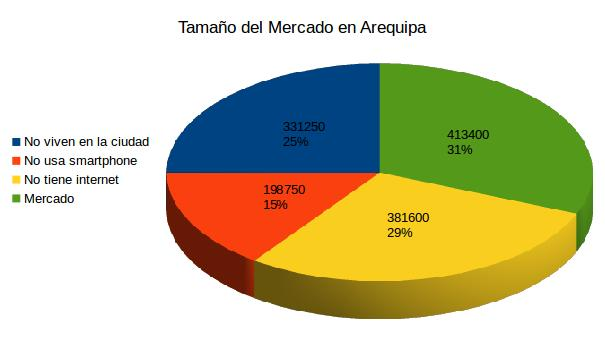
\includegraphics[width=0.7\textwidth]{img/mercado.jpg} 
  \caption{Tamaño del mercado en Arequipa}
  \label{fig:mercado}
\end{figure}

% gráficos
% aterrizarlo a la gente que usa servicio de courier

\subsubsection{Estacionalidad}
No existe estacionalidad en nuestro servicio, ya que se utiliza constantemente a lo largo del año.

\subsubsection{Tendencias del sector}
Cuando las personas necesitan enviar o traer un paquete, suelen optar por alguna de las siguientes alternativas, llevan o traen el paquete ellas mismas, o envían a alquien. Y si se trata de una empresa, entonces implementan su propia forma de delivery o simplemente no tienen delivery en absoluto.
% llevar el paquete
% recoger el paquete
% enviar a alguien de confianza con el paquete
% empresas: su propia forma de delivery


\subsubsection{Crecimiento potencial}
Contamos con dos formas de crecimiento potencial, la primera es captar más clientes en la ciudad de Arequipa y pasar de un 10\% que es la meta para el primer año a un 50\% en el año siguiente. Y la otra forma de crecimiento es expandirnos a más ciudades del país, siendo las más llamativas las ciudades de Lima y Trujillo.

\subsubsection{Infraestructura}
Como infraestructura física necesitamos una oficina donde nuestros desarrolladores programen la aplicación y un local donde se haga la verificación de los taxistas y los contratos con las empresas de taxi. Este local debe ser la cara de la compañía.
% Infraestructura computacional
Como infraestructura computacional, necesitamos para comenzar un servidor de Amazón EC2. Una base de datos Mongo conectada con Neo4j para guardar y procesar los datos y peticiones de los usuarios. También necesitaremos conectarnos a google maps para obtener el mapa de la ciudad y trazar las rutas de los taxis.
% local donde se reciban reclamos, se verifiquen los taxistas
% oficina de trabajo

\subsubsection{Precios del sector}
Los precios para las carreras de los taxis varían desde los 5 soles hasta los 20 aproximadamente. El precio de courier interprovincial con OLVA courier varía entre 20 y 100 soles. El precio de hacer envíos con taxitel es el mismo que el de transporte de personas. Y el precio de delivery de algunas empresas como pizzerias es gratuito a partir de cierto monto de compra (20 soles normalmente).
% precio de los taxis
% precio del mandadito
% precio de olva courier
% precio de delivery
% precio de taxitel courier

\subsubsection{Márgenes de la industria}
Es complicado calcular el margen de ganancia de los taxistas, puesto que depende de si el carro es propio o alquilado, si está hipotecado y ya está totalmente pagado. Depende del consumo del vehículo e incluso del tipo de conducción del taxista y el mantenimiento que se le brinda al vehículo.
% cuanto ganan los taxistas
% cuanto ganan olva courier, mandadito, taxitel, etc


\subsection{Análisis de las fuerzas competitivas de la industria}

\subsubsection{Proveedores y su poder de negociación}
Actualmente en Arequipa existe un poco mas de 25 mil taxis, de los cuales 20 mil tienen autorizaciones (entre Setare y permisos transitorios), lo cual nos indica que la demanda es muy alta. Por lo que el poder de negociación  no se vería tan afectado, obteniendo el costo de la comisión a nuestro favor. 
Otro proveedor grande serian los inversionistas; actualmente en el mercado existe competencia como Olva Currier, El mandadito, entre otros, por lo que el poder de negociación se vera en que es lo que nosotros ofrecemos en comparación a las demás empresas.

\subsubsection{Rivalidad entre las empresas que compiten en el mercado}
Actualmente existen en Arequipa mas de 10 empresas currier,entre los mas importantes se tienen a Olva currier, El mandadito, Taxitel, Expreso Marvisur, Locanto, Zapmeta, entre otros. Y el costo de sus servicios se da por medio del peso que se lleva,y la distancia acordada. Generalmente ellos mismos tienen sus movilidades de acuerdo para cada ocasión, ya sea camiones, motos, autos, o incluso hacer tramites para llevarlo al extranjero o interprovincial.Pero como toda empresa la mayoria entra al mercado con promociones por lo que tienden a disminuir sus precios, haciendo que las otras empresas se vean afectadas. 
Cada empresa guarda un prestigio, unas mas que otras, eso ayuda mucho al momento de competir en el mercado.

\subsubsection{Nuevos competidores y sus posibilidades de entrada}
Con lo referente a la posibilidad de nuevos competidores esta abierta, ya que cualquiera puede acceder a este servicio y hacer una copia de este servicio, o incluso mejorarla, pero lo que les sera difícil es conseguir los clientes, y su confianza, por lo que muchos tenderán a cerrar.
Algunas barreras de entrada que puede uno puede atravesar son:
\begin{itemize}
    \item La desconfianza de los clientes.
    \item Los precios bajos de otras empresas.
    \item La inseguridad de los clientes.
    \item Las capacidades en cuanto a peso, que no cubran el rango deseado. 
\end{itemize}

\subsubsection{Desarrollo de productos sustitutos}
Entre los productos sustitutos que pueden desfasar el nuestro, se tienen:
\begin{itemize}
    \item Los servicios de Taxi, que uno mismo puede llevar el producto.
    \item Confiar en un taxi conocido que lleve nuestros productos por nosotros.
    \item El servicio Currier de cada empresa.
\end{itemize}

\subsubsection{Compradores y su poder de negociación}
El comprador en este caso serian los clientes que pidan este servicio, ya sean personas naturales o empresas Pymes. La ventaja que se tiene es que los clientes no conocen muchas empresas que brinden este servicio, y si conocen, no son muchas las opciones que se tienen. Por lo que el poder de negociación seria bueno para nosotros una vez llegado al cliente (Persona Natural).
Pero en cuanto a Pymes, el poder de negociación, seria mayor , ya que hay encargados que se dedican a buscar por detalle estos servicios, buscando la mejor oferta, que sea eficiente y eficaz al mismo tiempo.
\section{Análisis interno}

\subsection{Análisis AMOFHIT}
\subsubsection{Administración y Gerencia}
La Gerencia se tendrá por dos personas, que serán quienes creen el producto, también se necesitara una persona de marketing que impulse el producto, para llegar a las personas naturales y a las empresas Pymes, y un administrador que nos ayude en ese campo, para que la empresa no se vaya a pique al momento de bajar precios o promocionar el producto. 

\subsubsection{Marketing y Ventas}
Para que el producto pueda salir al mercado y competir con grandes empresas se necesitara de un plan de marketing, que se vera reflejado en la publicidad por medio de la persona encargada. También es necesario entrar con promociones y bajos precios, que no afecten mucho a la economía de la empresa. Otro factor muy importante es que se tendrá acceso al software por medio del celular móvil, lo cual aumentara el posicionamiento del producto, llegando a personas que usan un SmartPhone.
Estos precios se verán reflejados en las comisiones tomadas por cada envió de acuerdo al peso enviado,a la distancia recorrida, al nivel de seguridad que se requiera.

\subsubsection{Operaciones Logísticas}
Dentro de los operaciones que se tendrá tenemos:
\begin{itemize}
    \item El cliente podra validarse una unica vez en su celular.
    \item La validación de un chofer al entrar a la empresa, sera efectuada por una persona encargada, estas entrevistas deberán ser efectuadas cara a cara con el conductor, y mediante una serie de pruebas se tomara la decisión si esta apto para ser uno de nuestros socios.
    \item Cada chofer contara con una cartilla de identificación, que tendrá que ser notoria a la vista del cliente. En esta cartilla figurara, el nombre del chofer, la placa del carro , la foto del chofer, el código único que sera brindado por la empresa.
    \item El chofer contara con un software diferente al del cliente en su celular, el cual le avisara si tiene un envió o no mediante notificaciones.
    \item El chofer contara con un mapa en su celular, que le dará la ubicación exacta del cliente, la ubicación del destino, y una posible vía rápida, esto se hará mediante google maps, por lo que el chofer tiene que estar conectado necesariamente a internet.
    \item El cliente por otro lado, tendrá un mapa en su celular que le permitirá conocer la ubicación actual de su paquete, así como las características del vehículo y del chofer.
    \item El cliente tendrá la información del pago a realizarse, esta información la brindara el chofer, y luego pasara por la empresa para aumentar la comisión respectiva. 
    \item El chofer tendrá acceso a este pago,y al finalizar el día, este tendrá el monto que deberá entregar a la empresa.
\end{itemize}

\subsubsection{Finanzas y Contabilidad}
Para financiar nuestro producto, se recaudara capital semilla de inversores y concursos Startups. Los gastos adicionales se vera por medio de los fundadores de la empresa. Todo esto mediante el departamento de contabilidad, para ver si se recupera lo invertido y que la empresa no este quebrando.

\subsubsection{Recursos Humanos}
Para conseguir trabajadores dentro de la empresa, se vera la posibilidad de contratar practicantes, con bajo salario en un principio a medio tiempo, con un perfil del tercio superior y ganas de aprender. Si es que la persona demuestra potencial, se le hará parte de la empresa.

En cuanto a los conductores, tendrán que ser personas responsables, que no tengan papeletas, ni problemas con la ley. Estas personas si demuestran fidelidad se les dará incentivos, por su merito al esfuerzo y su siempre disponibilidad.

\subsubsection{Sistema de información y Comunicaciones}
La comunicación en la empresa es algo fundamental; por si ocurre un incidente, el chofer comunicara a la empresa, para que esta pueda solucionar el incidente. Es por eso que es muy importante que el internet del conductor siempre este activo , ya que sera un medio importante por la cual fluya la comunicación, en caso el internet falle, por algún incidente, tendrá que comunicarse con la empresa vía telefónico.
La información del cliente sera enviada al conductor y al final del día, toda esa información sera llevada a la empresa vía virtual, para que se pueda hacer un análisis de los clientes que piden este servicio y comunicarles nuestras promociones.


\subsubsection{Tecnología Investigación y desarrollo}
El área de TI, sera el encargado de desarrollar software que mejore el servicio de paquetería o que amplié el campo laboral. Nuestros trabajos futuros serán:
\begin{itemize}
\item Software que permita con una foto tomada a la placa, ver todos los datos del carro y del conductor.
\item Software que permita enlazarnos con Siri, Cortana para hacer un pedido de movilidad por medio de voz
\item Permitir no solo el envió de paquetes, sino también el traslado de personas.
\item Permitir el uso compartido de un taxi o movilidad, por medio de una software que brinde la información de cada persona que comparte la movilidad.
\end{itemize}

\subsection{Recursos y capacidades de la empresa}
A continuación se muestra una tabla de recursos que conforman las capacidades de la empresa:

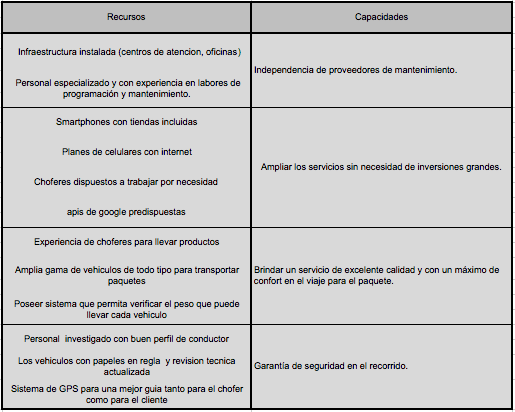
\includegraphics[width=0.8\textwidth]{tablaRyC}

\subsection{Ventaja competitiva actual}
A continuación se evalúa las ventajas competitivas que harán que la empresa tenga presencia empresarial:
\begin{itemize}
    \item La mayor parte de personas tiene un SmartPhone, por lo que llegar a ellos no sera tan difícil.
    \item El uso de apis de google con sistema de rastreo, ayudara a que las personas se sientan seguras, porque podrán hacer seguimiento a sus paquetes.
    \item El diseño amigable del software hará que la interacción entre el software y el usuario sea muy eficiente.
    \item Bajos costos de comisión, para poder entrar en el mercado.
    \item Utilización de los mismos conductores que hay en la ciudad de Arequipa.
\end{itemize}

\subsection{Estructura organizativa}
Actualmente se cuenta con una estructura lineal, ya que los gerente son los dueños, pero una vez organizado bien el software se contara con un sistema mono funcional como se ve en la imagen.

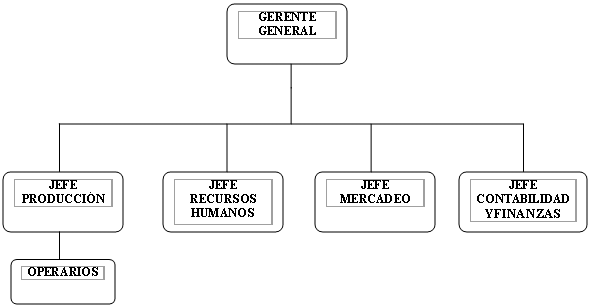
\includegraphics[width=0.8\textwidth]{planNegocios}
